\chapter{Całki zależne od parametrów}
\label{ma2:ch:parameter-integrals}

Niech $n,m\ge1$ będą liczbami naturalnymi,
$A\subseteq\R^n$ będzie mierzalny,
$T\subseteq\R^m$ i $f:T\times A\to\R$.
Przyjmujemy $v_n=\lambda_n(B(0,1))$, gdzie kule
są euklidesowe.
Rozpatrujemy funkcję skalarną
\[
 F(t)=\int_A f(t,x)\,\mathrm d\lambda_n(x).
\]
Zmienna $x$ jest zmienną całkowania, a $t$ parametrem.
Jeżeli nie zaznaczono inaczej, zakładamy mierzalność
każdego przekroju $x\mapsto f(t,x)$ i przez istnienie
całki rozumiemy całkowalność w sensie Lebesgue'a.
Jednowymiarowy rachunek całek Riemanna i całek
niewłaściwych omówiono w
\atlasref{AM1-32::ma1:ch:parameter-integrals}{AM I, rozdział 32},
a ogólną teorię miarową w
\atlasref{ME-11::ch:parametry-calki}{teorii miary i całki, rozdział 11}.
Tutaj rozwijamy rachunek dla parametrów euklidesowych.
Nie zakładamy jeszcze twierdzenia Fubiniego ani
wielowymiarowego wzoru na zamianę zmiennych.

\section{Intuicja: zmiana funkcji i zmiana dziedziny}

Dla ustalonego parametru $t$ funkcja
$f(t,\cdot)$ opisuje rozkład pewnej wielkości
na zbiorze $A$. Jeżeli przekrój jest całkowalny,
całka $F(t)$ jest jej łączną wartością ze znakiem. Zmiana
parametru może zmieniać wysokość funkcji,
jej nośnik, położenie osobliwości lub
samą dziedzinę całkowania. Należy odróżniać
te mechanizmy, ponieważ wymagają innych
oszacowań.

\paragraph{Ciągłość przy ustalonej dziedzinie.}
Jeżeli oba przekroje są całkowalne, to
z liniowości i oszacowania modułu całki
(\ref{ma2:thm:lebesgue-linearity}) otrzymujemy
\[
 |F(t)-F(t_0)|\le
 \int_A |f(t,x)-f(t_0,x)|\,\mathrm d\lambda_n(x).
\]
Ciągłość punktowa przekrojów względem
$t$ nie wystarcza do zapewnienia, że
prawa strona dąży do zera. Wkład może
przesuwać się w nieskończoność lub
skupiać na coraz mniejszym zbiorze.
Przykłady takich zjawisk widzieliśmy
w \ref{ma2:ex:lebesgue-concentration}.
Wspólna całkowalna majoranta wyklucza
obie trudności; ścisłym narzędziem jest
twierdzenie o zbieżności zmajoryzowanej
\ref{ma2:thm:lebesgue-dominated}.
Nie musi to być stała: na nieograniczonym
zbiorze stałe dodatnie mogą w ogóle
nie być całkowalne.

\paragraph{Różniczkowanie pod znakiem całki.}
Dla parametru rzeczywistego, gdy $t,t+h\in T$,
$h\ne0$ i oba przekroje są całkowalne,
liniowość daje
\[
 \frac{F(t+h)-F(t)}h
 =\int_A\frac{f(t+h,x)-f(t,x)}h\,
       \mathrm d\lambda_n(x).
\]
Punktowa granica ilorazu różnicowego
to $\partial_t f(t,x)$ tam, gdzie
pochodna istnieje. Aby przenieść granicę
pod całkę, potrzebujemy kontroli tych
ilorazów. Jeżeli funkcja parametru jest różniczkowalna
na otwartym przedziale zawierającym
cały krótki odcinek parametrów
i spełniają $|\partial_t f(s,x)|\le g(x)$
dla całkowalnej $g$, to twierdzenie
o wartości średniej daje
\[
 \left|\frac{f(t+h,x)-f(t,x)}h\right|\le g(x).
\]
Założenia te rozumiemy poza wspólnym
zbiorem miary zero. Stosując zbieżność
zmajoryzowaną wzdłuż dowolnego ciągu
$h\to0$, otrzymujemy wzór na $F'(t)$.
Pełna wersja wielowymiarowa znajduje się
w twierdzeniu \ref{ma2:thm:parameter-multivariate}.
Majoranta samej funkcji $f$ nie daje
automatycznie majoranty ilorazów różnicowych.

\paragraph{Zmiana dziedziny.}
Niech $A_t$ będzie rodziną zbiorów
mierzalnych, a $u(t,\cdot)$ funkcją
określoną na całej przestrzeni.
Wtedy
\[
 F(t)=\int_{\R^n}\chi_{A_t}(x)u(t,x)\,
                   \mathrm d\lambda_n(x).
\]
Przy całkowalności przekrojów na ich
odpowiednich dziedzinach różnicę $F(t+h)-F(t)$ można rozłożyć
na zmianę gęstości na części wspólnej
oraz wkłady z części dodanej i usuniętej:
\[
 \begin{aligned}
 F(t+h)-F(t)
 ={}&\int_{A_{t+h}\cap A_t}
      (u(t+h,x)-u(t,x))\,\mathrm d\lambda_n(x)\\
 &+\int_{A_{t+h}\setminus A_t}
      u(t+h,x)\,\mathrm d\lambda_n(x)\\
 &-\int_{A_t\setminus A_{t+h}}
      u(t,x)\,\mathrm d\lambda_n(x).
 \end{aligned}
\]
Równość wynika z rozkładu obu dziedzin
na rozłączne części i liniowości całki.
W przypadku funkcji ciągłych i
ograniczonych na wspólnym zwartym
otoczeniu ruchomych zbiorów każdy
z tych składników jest określony.
W szczególności nie wystarcza
różniczkowanie samej funkcji podcałkowej,
gdy dziedzina zależy od parametru.

\begin{przyklad}[Dwa źródła zmiany całki]
\label{ma2:ex:parameter-two-changes}
Dla $t>0$ rozważmy
\[
 F(t)=\int_{[0,t]}(1+tx)\,\mathrm d\lambda_1(x)
      =t+\frac{t^3}{2}.
\]
Ostatnia równość wynika ze wzoru
Newtona--Leibniza
(\ref{ma2:thm:primitive-newton-leibniz})
i zgodności całek Riemanna i Lebesgue'a.
Stąd $F'(t)=1+3t^2/2$.
Dla $h>0$ rozkład różnicy daje
\[
 F(t+h)-F(t)
 =h\int_{[0,t]}x\,\mathrm d\lambda_1(x)
 +\int_{[t,t+h]}(1+(t+h)x)\,\mathrm d\lambda_1(x).
\]
Wspólny koniec przedziałów ma miarę zero.
Pierwszy składnik po podzieleniu przez $h$
jest równy $t^2/2$. Drugi po podzieleniu
przez $h$ dąży do $1+t^2$, ponieważ
dla $x\in[t,t+h]$ mamy
$|(t+h)x-t^2|\le 2th+h^2$, co dąży do zera.
Dla $h<0$ i $t+h>0$ otrzymujemy
analogicznie
\[
 \frac{F(t+h)-F(t)}h
 =\int_{[0,t+h]}x\,\mathrm d\lambda_1(x)
 +\frac1{|h|}\int_{[t+h,t]}(1+tx)\,
                                    \mathrm d\lambda_1(x).
\]
Oba składniki mają te same granice
co poprzednio. Widzimy więc osobno
zmianę wartości funkcji w dotychczasowej
dziedzinie i zmianę wynikającą z ruchu
jej brzegu:
\[
 F'(t)=\underbrace{\frac{t^2}{2}}_{\text{zmiana gęstości}}
       +\underbrace{1+t^2}_{\text{zmiana dziedziny}}.
\]
To szczególny przypadek reguły Leibniza,
do której powrócimy w dalszej części rozdziału.
\end{przyklad}

\begin{figure}[htbp]
\centering
\begin{tikzpicture}[x=4.2cm,y=1.65cm,>=stealth]
 \fill[blue!20] (0,0)--(0,1)--(1,2)--(1,0)--cycle;
 \filldraw[fill=teal!55,draw=teal!80!black]
 (0,1)--(1,2)--(1,2.25)--cycle;
 \filldraw[fill=orange!50,draw=orange!85!black]
 (1,0)--(1,2.25)--(1.25,2.5625)--(1.25,0)--cycle;
 \draw[blue!75!black,thick] (0,1)--(1,2);
 \draw[teal!80!black,thick] (0,1)--(1.25,2.5625);
 \draw[->,gray!80!black] (-.05,0)--(1.53,0) node[right] {$x$};
 \draw[->,gray!80!black] (0,-.08)--(0,2.94) node[above] {$u(t,x)$};
 \draw[densely dashed,gray] (1,0)--(1,2.25);
 \draw[densely dashed,gray] (1.25,0)--(1.25,2.5625);
 \node[below] at (0,0) {$0$};
 \node[below] at (1,0) {$t$};
 \node[below] at (1.25,0) {$t+h$};
 \node[blue!75!black] at (.52,.63) {$F(t)$};
 \draw[teal!80!black,<-] (.65,1.73)--(.54,2.67)
 node[above] {\small zmiana gęstości};
 \draw[orange!85!black,<-] (1.13,1.12)--(1.43,1.12)
 node[right] {\small ruch brzegu};
\end{tikzpicture}
\caption{Przyrost całki z przykładu
\ref{ma2:ex:parameter-two-changes} dla $t=1$
i $h=1/4$. Niebieskie pole to dotychczasowa
całka, zielony trójkąt odpowiada zmianie
gęstości, a pomarańczowy trapez zmianie
dziedziny.}
\label{ma2:fig:parameter-two-changes}
\end{figure}

\section{Ciągłość całki i lokalne majoranty}

\begin{twierdzenie}[Ciągłość całki względem parametrów]
\label{ma2:thm:parameter-continuity}
Niech $t_0\in T$. Załóżmy, że dla prawie każdego
$x\in A$ funkcja $f(\cdot,x)$ jest ciągła w $t_0$,
a w pewnym względnym otoczeniu $V$ punktu $t_0$
istnieje nieujemna całkowalna funkcja $g:A\to\R$
taka, że $|f(t,x)|\le g(x)$ dla wszystkich $t\in V$
i wszystkich $x$ poza wspólnym zbiorem miary zero.
Wtedy $F$ istnieje na $V$ oraz
\[
 \lim_{t\to t_0}\int_A |f(t,x)-f(t_0,x)|
 \,\mathrm d\lambda_n(x)=0.
\]
W szczególności $F$ jest ciągła w $t_0$.
\end{twierdzenie}
Jest to specjalizacja wyników
\atlasref{ME-11::thm:local-continuity-11}{o ciągłości całki}
oraz
\atlasref{ME-11::cor:l1-param-11}{o ciągłości w normie $L^1$}
do miary Lebesgue'a ograniczonej do $A$.
Nie jest potrzebna jedna majoranta na całym $T$.
W istocie w warunku majoranty można dopuścić
zbiór wyjątkowy zależny od $t$: dla dowolnego
ciągu $t_j\to t_0$ wystarczy usunąć przeliczalną
sumę zbiorów wyjątkowych dla $t_0,t_1,t_2,\ldots$.
Na pozostałej części $A$ różnice są zmajoryzowane
przez $2g$ i zbiegają punktowo do zera, więc
zbieżność zmajoryzowana daje żądaną granicę.
Nie należy stosować tego argumentu bezpośrednio
do nieprzeliczalnej rodziny parametrów w dowodzie
oszacowania pochodnej przez twierdzenie o wartości
średniej: tam potrzebujemy kontroli na całym odcinku.

\begin{wniosek}[Całka na zwartym zbiorze Jordana]
\label{ma2:cor:parameter-riemann-compact}
Jeżeli $A$ jest zwarty i mierzalny w sensie Jordana,
a $f:T\times A\to\R$ jest ciągła, to $F$ jest ciągła.
Całka może być rozumiana również jako całka Riemanna.
\end{wniosek}
\begin{proof}
Dla ustalonego $t_0$ i dowolnego ciągu $t_j\to t_0$
w $T$, zbiór $K=\{t_0,t_1,t_2,\ldots\}$ jest zwarty.
Ciągłość na zwartym $K\times A$ daje ograniczenie
$|f|\le M$. Stała $M$ na $A$ jest całkowalna,
gdyż $A$ jest ograniczony. Twierdzenie o zbieżności
zmajoryzowanej \ref{ma2:thm:lebesgue-dominated}
daje $F(t_j)\to F(t_0)$.
Zgodność obu całek wynika z
\ref{ma2:thm:lebesgue-jordan-agreement}.
\end{proof}

\section{Różniczkowanie względem wielu parametrów}

\begin{twierdzenie}[Pochodne całki]
\label{ma2:thm:parameter-multivariate}
Niech $T\subseteq\R^m$ będzie otwarty,
a $k\ge1$ będzie liczbą naturalną.
Załóżmy, że $f(t,\cdot)$ jest całkowalna dla każdego
$t\in T$, a poza ustalonym mierzalnym zbiorem zerowym
$N\subseteq A$ funkcje $f(\cdot,x)$ są klasy $C^k$.
Dla każdej domkniętej kuli $K\subset T$
i każdego wielowskaźnika $\alpha$ z
$1\le|\alpha|\le k$ niech istnieje nieujemna
całkowalna funkcja $g_{K,\alpha}$ taka, że
\[
 |\partial_t^\alpha f(t,x)|\le g_{K,\alpha}(x)
 \qquad(t\in K,\ x\in A\setminus N).
\]
Wtedy $F\in C^k(T)$ oraz
\[
 \partial^\alpha F(t)=\int_A \partial_t^\alpha f(t,x)
 \,\mathrm d\lambda_n(x)
 \qquad (1\le|\alpha|\le k).
\]
Na $N$ przyjmujemy wszystkie pochodne podcałkowe
równe zero.
\end{twierdzenie}
\begin{proof}
Ustalmy $t_0\in T$ i domkniętą kulę $K$
o środku $t_0$ i dodatnim promieniu, zawartą w $T$.
Każdy przekrój pochodnej jest mierzalny: dla
pierwszych pochodnych jest to granica mierzalnych
ilorazów różnicowych wzdłuż ciągu niezerowych
przyrostów dążących do zera, poza $N$; dla wyższych
pochodnych powtarzamy ten argument.
Na mierzalnym $N$ określamy granice przez zero.

Dla pierwszej pochodnej ograniczamy parametr do
odcinka $t+s e_i$ zawartego w $K$, gdzie $e_i$
jest $i$-tym wektorem bazy standardowej.
Hipotezy
\atlasref{ME-11::thm:local-differentiation-11}{lokalnego twierdzenia o różniczkowaniu}
są spełnione w każdym punkcie wnętrza $K$:
przekrój początkowy jest całkowalny, pochodna
istnieje poza $N$ i ma majorantę $g_{K,e_i}$.
Otrzymujemy wzór dla $\partial_i F$.
Dla $\partial_t^\alpha f$ z $1\le|\alpha|<k$
stosujemy to samo rozumowanie, używając
całkowalności wynikającej z $g_{K,\alpha}$
oraz majoranty $g_{K,\alpha+e_i}$.
Indukcja daje wszystkie żądane wzory, niezależnie
od kolejności różniczkowania: pochodne mieszane
funkcji klasy $C^k$ można permutować na mocy
twierdzenia \ref{ma2:thm:schwarz}.
Ciągłość pochodnych wynika z
\ref{ma2:thm:parameter-continuity}, ponieważ
odpowiednie pochodne podcałkowe są ciągłe w $t$
poza $N$ i lokalnie zmajoryzowane.
Z kryterium ciągłych pochodnych częściowych
\ref{ma2:thm:continuous-block-partials},
stosowanego do współrzędnych (a następnie do
pochodnych niższych rzędów), wynika $F\in C^k$.
Ponieważ
$t_0$ był dowolny, teza zachodzi na $T$.
\end{proof}

\begin{wniosek}[Całkowalność w jednym punkcie każdej składowej]
\label{ma2:cor:parameter-anchor}
W twierdzeniu \ref{ma2:thm:parameter-multivariate}
wystarczy założyć całkowalność $f(t_*,\cdot)$
dla co najmniej jednego $t_*$ w każdej składowej
spójnej zbioru $T$, zamiast dla każdego $t\in T$.
\end{wniosek}
\begin{proof}
Niech $K$ będzie domkniętą kulą zawartą w $T$.
Dla $s,t\in K$ i $x\notin N$ stosujemy
twierdzenie o wartości średniej do funkcji
$\theta\mapsto f(s+\theta(t-s),x)$ na $[0,1]$.
Reguła łańcuchowa i ograniczenia pochodnych dają
\[
 |f(t,x)-f(s,x)|\le
 \sum_{i=1}^m |t_i-s_i|g_{K,e_i}(x).
\]
Prawa strona jest całkowalna jako skończona suma
funkcji całkowalnych. Zatem wszystkie przekroje
na $K$ są jednocześnie całkowalne albo wszystkie
niecałkowalne. Każdy punkt $T$ ma takie kuliste
otoczenie, więc zbiór parametrów o całkowalnym
przekroju oraz jego dopełnienie są otwarte w $T$.
Na składowej spójnej zawierającej $t_*$ pierwszy
zbiór jest niepusty, wobec czego obejmuje całą
składową. Stosujemy poprzednie twierdzenie.
\end{proof}

\begin{wniosek}[Gradient, macierz Hessego i różniczka]
\label{ma2:cor:parameter-gradient-hessian}
Przy założeniach twierdzenia
\ref{ma2:thm:parameter-multivariate} (również
z osłabieniem z wniosku \ref{ma2:cor:parameter-anchor})
dla $k\ge1$ mamy, współrzędna po współrzędnej,
\[
 \nabla F(t)=\left(
 \int_A\partial_{t_i}f(t,x)\,\mathrm d\lambda_n(x)
 \right)_{i=1}^m,
\]
a dla $h\in\R^m$
\[
 DF(t)[h]=\int_A
 \left(\sum_{i=1}^m h_i\partial_{t_i}f(t,x)\right)
 \,\mathrm d\lambda_n(x).
\]
Jeżeli $k\ge2$, to
\[
 H_F(t)=\left(
 \int_A\partial_{t_i}\partial_{t_j}f(t,x)
 \,\mathrm d\lambda_n(x)
 \right)_{i,j=1}^m.
\]
\end{wniosek}
\begin{proof}
Stosujemy wzory na pochodne cząstkowe z
\ref{ma2:thm:parameter-multivariate} oraz
współrzędnościowe przedstawienie różniczki
funkcji klasy $C^1$ z twierdzenia
\ref{ma2:thm:continuous-block-partials}.
Skończoną sumę przenosimy pod znak całki
na mocy liniowości. Macierz Hessego otrzymujemy,
stosując wzór dla wielowskaźników rzędu dwa.
Nie korzystamy z całkowania wektorowego.
\end{proof}

\begin{przyklad}[Całka radialna z dwoma parametrami]
\label{ma2:ex:parameter-radial-exponential}
Dla $a>0$, $b>0$ rozważmy
\[
 F(a,b)=\int_{\R^n}
 \exp(-a\|x\|_2-b)\,\mathrm d\lambda_n(x).
\]
Ze wzoru radialnego \ref{ma2:thm:improper-radial}
wynika
\[
 F(a,b)=nv_n e^{-b}\int_0^\infty
 r^{n-1}e^{-ar}\,\mathrm d\lambda_1(r)
 =v_n n! e^{-b}a^{-n}.
\]
Ostatnią równość otrzymujemy przez podstawienie
$u=ar$ i wzór $\int_0^\infty u^{n-1}e^{-u}
\,\mathrm d\lambda_1(u)=(n-1)!$,
wynikający z całkowania przez części (por.
\atlasref{ME-11::ex:gamma-param-11}{funkcja Gamma}).
Dla każdego zwartego zbioru parametrów
z $a\ge a_0>0$, $b>0$ pochodne rzędu $j+\ell$
są zmajoryzowane przez $\|x\|_2^j e^{-a_0\|x\|_2}$.
Całkowalność tych majorant wynika z tego samego
wzoru radialnego.
Twierdzenie \ref{ma2:thm:parameter-multivariate}
daje zatem
\[
 \int_{\R^n}\|x\|_2^j e^{-a\|x\|_2-b}
 \,\mathrm d\lambda_n(x)
 =nv_n e^{-b}\frac{(n+j-1)!}{a^{n+j}}
 \qquad(j=0,1,2,\ldots).
\]
Można to uzyskać przez $j$-krotne różniczkowanie
$F$ względem $a$ i pomnożenie wyniku przez $(-1)^j$.
\end{przyklad}

\begin{przyklad}[Parametr w wykładniku osobliwości]
\label{ma2:ex:parameter-singularity}
Niech $p<n$ i
\[
 G(p)=\int_{\{0<\|x\|_2<1\}}\|x\|_2^{-p}
 \,\mathrm d\lambda_n(x)=\frac{nv_n}{n-p}.
\]
Równość wynika z \ref{ma2:ex:improper-radial-power}
przez przejście z dolnym promieniem do zera.
Dla zwartego przedziału parametrów z $p\le b<n$
pochodna rzędu $j$ jest ograniczona przez
$r^{-b}(\log(1/r))^j$ przy $r=\|x\|_2\in(0,1)$.
Wzór radialny i podstawienie $u=\log(1/r)$ dają
całkę majoranty równą
$nv_n\int_0^\infty e^{-(n-b)u}u^j
\,\mathrm d\lambda_1(u)<\infty$.
Stąd dla $j\ge0$
\[
 \int_{\{0<\|x\|_2<1\}}
 \frac{(\log(1/\|x\|_2))^j}{\|x\|_2^p}
 \,\mathrm d\lambda_n(x)
 =\frac{nv_n j!}{(n-p)^{j+1}}.
\]
Wzór otrzymujemy przez różniczkowanie $G$.
Przy $p\uparrow n$ całka podstawowa i wszystkie
te momenty logarytmiczne dążą do nieskończoności.
\end{przyklad}

\begin{przyklad}[Gładkie przekroje nie gwarantują różniczkowalności całki]
\label{ma2:ex:parameter-escape-derivative}
Niech $\psi:\R^n\to[0,\infty)$ będzie ciągłą
funkcją klasy $C^\infty$, równą zero poza kulą
domkniętą jednostkową, o całce równej $1$.
Można ją uzyskać, normalizując funkcję
\[
 \psi_0(x)=
 \begin{cases}
 \exp(-1/(1-\|x\|_2^2)),&\|x\|_2<1,\\
 0,&\|x\|_2\ge1.
 \end{cases}
\]
Jej całka jest dodatnia i skończona, ponieważ
funkcja jest ograniczona, ma ograniczony nośnik
i jest dodatnia we wnętrzu kuli.
Gładkość na brzegu wynika z faktu, że funkcja
$s\mapsto e^{-1/s}$ dla $s>0$, przedłużona zerem
dla $s\le0$, jest gładka. Indukcyjnie, stosując
regułę iloczynu i łańcuchową, otrzymujemy na
dodatniej półosi pochodne postaci $P(1/s)e^{-1/s}$,
gdzie $P$ jest wielomianem. Każde takie wyrażenie
oraz jego iloraz przez $s$ dążą do zera przy
$s\downarrow0$, ponieważ wykładnicza funkcja
zanika szybciej od każdej potęgi $s$.
Indukcja wprost z definicji pochodnej w zerze
pokazuje, że wszystkie pochodne przedłużenia
istnieją i są tam równe zero. Gładkość $\psi_0$
wynika następnie z reguły łańcuchowej.

Dla $t\in(-1,1)$ określmy
\[
 f(t,x)=
 \begin{cases}
 |t|\psi(x-e_1/t),&t\ne0,\\
 0,&t=0.
 \end{cases}
\]
Funkcja jest gładka również w otoczeniu każdego
punktu $(0,x_0)$: dla $x$ w ograniczonym otoczeniu
$x_0$ i dostatecznie małego $|t|$ zachodzi
$\|x-e_1/t\|_2>1$, więc $f$ jest tam identycznie
zerowa. W szczególności $\partial_t f(0,x)=0$
dla każdego $x$.
Niezmienniczość miary względem translacji
(\atlasref{ME-04::thm:invariance-lebesgue}{teoria miary i całki}),
przeniesiona z funkcji charakterystycznych na
nieujemne funkcje przez aproksymację prostą
i zbieżność monotoniczną, daje
\[
 F(t)=\int_{\R^n}f(t,x)\,\mathrm d\lambda_n(x)=|t|.
\]
Funkcja $F$ jest ciągła, lecz nie jest
różniczkowalna w zerze, mimo że wszystkie
pochodne przekrojów istnieją.
Gdyby pierwsza pochodna podcałkowa miała
wspólną całkowalną majorantę w otoczeniu zera,
twierdzenie \ref{ma2:thm:parameter-multivariate}
zastosowane po ograniczeniu przestrzeni parametrów
do mniejszego otwartego przedziału wokół zera
dawałoby różniczkowalność $F$ i $F'(0)=0$,
co jest sprzecznością.
Także sama rodzina $f(t,\cdot)$ nie ma wspólnej
całkowalnej majoranty w żadnym otoczeniu zera.
Istotnie, dla $t_j=1/(3j)$ oraz
$x\in B(3je_1,1/2)$ mamy $f(t_j,x)\ge c/(3j)$,
gdzie $c=\min_{\|y\|_2\le1/2}\psi(y)>0$.
Kule te są parami rozłączne i każda ma miarę
$v_n2^{-n}$. Gdyby $g$ była wspólną majorantą
(nawet z osobnym zbiorem wyjątkowym dla każdego
$t_j$), to dla dostatecznie dużego $J$ i $M\ge J$
\[
 \int_{\R^n}g\,\mathrm d\lambda_n
 \ge \frac{cv_n}{3\cdot 2^n}\sum_{j=J}^M\frac1j.
\]
Rozbieżność szeregu harmonicznego daje sprzeczność.
\end{przyklad}

\begin{figure}[htbp]
\centering
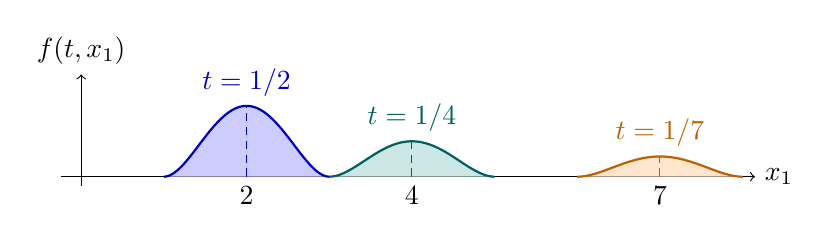
\begin{tikzpicture}[x=1.05cm,y=1cm]
 \draw[->] (-.25,0)--(8.15,0) node[right] {$x_1$};
 \draw[->] (0,-.12)--(0,1.3) node[above] {$f(t,x_1)$};
 \foreach \a/\h/\col in {2/.9/blue,4/.45/teal,7/.257/orange}{
   \fill[\col!20] plot[domain=-1:1,samples=60,variable=\s]
    ({\a+\s},{\h*(1-\s*\s)^2}) -- cycle;
   \draw[\col!75!black,thick] plot[domain=-1:1,samples=60,variable=\s]
    ({\a+\s},{\h*(1-\s*\s)^2});
   \draw[\col!75!black,densely dashed] (\a,0)--(\a,\h);
 }
 \node[below] at (2,0) {$2$};
 \node[below] at (4,0) {$4$};
 \node[below] at (7,0) {$7$};
 \node[blue!75!black,above] at (2,.9) {$t=1/2$};
 \node[teal!75!black,above] at (4,.45) {$t=1/4$};
 \node[orange!75!black,above] at (7,.257) {$t=1/7$};
\end{tikzpicture}
\caption{Schemat przesuwającego się nośnika z przykładu
\ref{ma2:ex:parameter-escape-derivative} dla $t>0$
i $n=1$. Kształt krzywych jest schematyczny;
środki są równe $1/t$, a wysokości proporcjonalne do $t$.}
\label{ma2:fig:parameter-escape}
\end{figure}

\begin{przyklad}[Majoranta funkcji nie zastępuje majoranty pochodnej]
\label{ma2:ex:parameter-bounded-concentration}
Niech $A=(0,1)$, $T=(-1/3,1/3)$, a $\eta$ będzie
nieujemną funkcją gładką na $\R$, o nośniku
zawartym w $[1,2]$ i całce równej $1$.
Taką funkcję otrzymujemy przez przesunięcie,
przeskalowanie i normalizację jednowymiarowej
funkcji $\psi_0$ z przykładu
\ref{ma2:ex:parameter-escape-derivative}.
Połóżmy
\[
 f(t,x)=
 \begin{cases}
 \eta(x/|t|),&t\ne0,\\
 0,&t=0.
 \end{cases}
\]
Dla ustalonego $x_0>0$ funkcja $f$ jest identycznie
zerowa w pewnym otoczeniu $(0,x_0)$, ponieważ
$x/|t|>2$ dla $x>x_0/2$ i $|t|<x_0/4$.
Poza $t=0$ jest gładka z reguły łańcuchowej.
Zatem $f\in C^\infty(T\times A)$ i
$\partial_t f(0,x)=0$ dla każdego $x\in A$.
W odróżnieniu od poprzedniego przykładu wszystkie
funkcje $f(t,\cdot)$ mają wspólną całkowalną
majorantę $\|\eta\|_\infty$ na $A$.
Całka $F$ jest więc ciągła na mocy
\ref{ma2:thm:parameter-continuity}.
Jednak dla $t\ne0$, podstawiając $s=x/|t|$,
otrzymujemy
\[
 F(t)=|t|\int_0^{1/|t|}\eta(s)\,
 \mathrm d\lambda_1(s)=|t|,
\]
gdyż $1/|t|>3$ i cały nośnik $\eta$
mieści się w przedziale całkowania.
Zatem $F$ nie ma pochodnej w zerze.
Istnienie majoranty funkcji podcałkowej
nie zapewnia przeniesienia różniczkowania pod całkę,
nawet na ograniczonym przedziale i przy
gładkości funkcji we wszystkich zmiennych
na otwartym zbiorze $T\times A$.
\end{przyklad}

\section{Zmienna dziedzina całkowania}

\begin{twierdzenie}[Ciągłość całki na ruchomych zbiorach]
\label{ma2:thm:parameter-moving-domains}
Niech $t_0\in T$, zbiory $A_t\subseteq\R^n$
będą mierzalne, a
$u:T\times\R^n\to\R$ ma mierzalne przekroje.
Załóżmy, że przy $t\to t_0$ zachodzi
\[
 \chi_{A_t}(x)u(t,x)\to
 \chi_{A_{t_0}}(x)u(t_0,x)
 \quad\text{dla prawie każdego }x.
\]
Jeżeli w pewnym otoczeniu $t_0$ istnieje
nieujemna całkowalna majoranta $g$ na $\R^n$
taka, że dla każdego $t$ z tego otoczenia
$|\chi_{A_t}u(t,\cdot)|\le g$ prawie wszędzie,
to $F(t)=\int_{A_t}u(t,x)\,\mathrm d\lambda_n(x)$
jest dobrze określona w tym otoczeniu i ciągła w $t_0$.
\end{twierdzenie}
Jest to szczególny przypadek
\atlasref{ME-11::thm:moving-domains-11}{twierdzenia o zmiennej dziedzinie}
dla miary Lebesgue'a; zbiór zerowy w warunku
majoranty może zależeć od parametru.

\begin{przyklad}[Kula o zmiennym środku i promieniu]
\label{ma2:ex:parameter-moving-ball}
Niech $u:\R^n\to\R$ będzie ciągła. Funkcja
\[
 H(c,r)=\int_{B(c,r)}u(x)\,\mathrm d\lambda_n(x),
 \qquad c\in\R^n,\quad r>0,
\]
jest ciągła. Istotnie, jeśli $(c,r)\to(c_0,r_0)$,
to $\|x-c\|_2-r\to\|x-c_0\|_2-r_0$.
Poza sferą o środku $c_0$ i promieniu $r_0$
znak tego wyrażenia jest ostatecznie stały,
więc funkcje charakterystyczne kul zbiegają
punktowo poza zbiorem zerowym (zerowość sfery
wynika z argumentu poprzedzającego
\ref{ma2:thm:improper-radial} i niezmienniczości
miary względem przesunięć).
W otoczeniu $(c_0,r_0)$ wszystkie kule mieszczą się
w pewnej kuli domkniętej $K$, na której $|u|\le M$.
Majorantą jest $M\chi_K$.
Stosujemy \ref{ma2:thm:parameter-moving-domains}.
\end{przyklad}

\begin{stwierdzenie}[Różniczkowanie położenia kuli]
\label{ma2:prop:parameter-ball-center}
Niech $u\in C^k(\R^n)$, $k\ge1$, i niech $r>0$
będzie ustalony. Wówczas funkcja
$H_r(c)=\int_{B(c,r)}u(x)\,\mathrm d\lambda_n(x)$
jest klasy $C^k$, a dla $1\le|\alpha|\le k$
\[
 \partial_c^\alpha H_r(c)
 =\int_{B(c,r)}\partial^\alpha u(x)\,
 \mathrm d\lambda_n(x).
\]
\end{stwierdzenie}
\begin{proof}
Niezmienniczość miary Lebesgue'a względem translacji
(\atlasref{ME-04::thm:invariance-lebesgue}{teoria miary i całki})
daje
\[
 H_r(c)=\int_{B(0,r)}u(c+y)\,\mathrm d\lambda_n(y).
\]
Wzór dla całek wynika z niezmienniczości dla
funkcji charakterystycznych, liniowości,
aproksymacji nieujemnych funkcjami prostymi
i rozkładu na część dodatnią i ujemną.
Dla $c$ w domkniętej kuli $K$ pochodne
$\partial^\alpha u(c+y)$ są ograniczone,
gdyż $K+\overline{B(0,r)}$ jest zwarty
jako obraz iloczynu dwóch zbiorów zwartych
przez ciągłe dodawanie. Stałe ograniczenia
są całkowalnymi majorantami na $B(0,r)$.
Twierdzenie \ref{ma2:thm:parameter-multivariate}
daje wzory pochodnych, a ponowne przesunięcie
zmiennej całkowania prowadzi do tezy.
\end{proof}

\begin{przyklad}[Moment drugiego rzędu ruchomej kuli]
\label{ma2:ex:parameter-ball-moment}
Dla $u(x)=\|x\|_2^2$ rozwinięcie kwadratu
po przesunięciu kuli daje
\[
 H_r(c)=v_nr^n\|c\|_2^2+
 \frac{nv_n}{n+2}r^{n+2}.
\]
Istotnie, $\|c+y\|_2^2=\|c\|_2^2+2\langle c,y\rangle+
\|y\|_2^2$, całka składnika liniowego po kuli
$B(0,r)$ jest zerowa dzięki symetrii $y\mapsto-y$,
a pozostały moment radialny obliczamy z
\ref{ma2:thm:improper-radial}.
Stąd $\nabla_c H_r(c)=2v_nr^n c$ oraz
$H_{H_r}(c)=2v_nr^n I_n$, gdzie $I_n$ jest
macierzą jednostkową. Wzory te można także
uzyskać bez obliczania samej całki:
stosujemy \ref{ma2:prop:parameter-ball-center}
do pochodnych $2x_i$ oraz $2\delta_{ij}$,
a następnie używamy tej samej symetrii.
\end{przyklad}

\begin{stwierdzenie}[Jednoczesna zmiana środka, promienia i gęstości]
\label{ma2:prop:parameter-ball-all}
Niech $I\subseteq\R$ będzie otwartym przedziałem,
$c:I\to\R^n$ i $r:I\to(0,\infty)$ będą klasy $C^1$,
a $u\in C^1(I\times\R^n)$. Dla
\[
 G(t)=\int_{B(c(t),r(t))}u(t,x)\,\mathrm d\lambda_n(x)
\]
mamy $G\in C^1(I)$ oraz, pisząc
$V(t,x)=c'(t)+\dfrac{r'(t)}{r(t)}(x-c(t))$,
\[
 \begin{aligned}
 G'(t)=\int_{B(c(t),r(t))}
 \bigg(&\partial_t u(t,x)+
 \langle\nabla_x u(t,x),V(t,x)\rangle\\
 &+\frac{nr'(t)}{r(t)}u(t,x)\bigg)
 \,\mathrm d\lambda_n(x).
 \end{aligned}
\]
\end{stwierdzenie}
\begin{proof}
Przenosimy całkowanie na ustaloną kulę jednostkową
za pomocą podobieństwa $x=c(t)+r(t)y$.
Niezmienniczość względem translacji i skalowanie
miary Lebesgue'a
(\atlasref{ME-04::thm:invariance-lebesgue}{ME 04})
dają
\[
 G(t)=r(t)^n\int_{B(0,1)}
 u(t,c(t)+r(t)y)\,\mathrm d\lambda_n(y).
\]
Tożsamość dla całek wynika z odpowiedniej
tożsamości miar dla funkcji charakterystycznych,
a następnie z aproksymacji funkcjami prostymi
i rozkładu na części dodatnią i ujemną.
Dla $t$ w dowolnym zwartym podprzedziale
zawartym w $I$ wszystkie argumenty $(t,c(t)+r(t)y)$,
$\|y\|_2\le1$, należą do jednego zbioru
zwartego. Funkcja podcałkowa i jej pochodna
względem $t$ są więc jednostajnie ograniczone
przez stałe całkowalne na $B(0,1)$.
Twierdzenie \ref{ma2:thm:parameter-multivariate}
oraz reguła iloczynu i reguła łańcuchowa dają
\[
 \begin{aligned}
 G'(t)={}&nr(t)^{n-1}r'(t)
 \int_{B(0,1)}u(t,c(t)+r(t)y)\,\mathrm d\lambda_n(y)\\
 &+r(t)^n\int_{B(0,1)}
 \big(\partial_t u(t,c(t)+r(t)y)\\
 &\hspace{3em}+\langle\nabla_x u(t,c(t)+r(t)y),
 c'(t)+r'(t)y\rangle\big)\,\mathrm d\lambda_n(y).
 \end{aligned}
\]
Ponownie stosując podobieństwo,
otrzymujemy żądany wzór.
\end{proof}

Pole $V$ opisuje prędkość punktów
poruszających się razem z kulą. Jego
dywergencja względem $x$ jest równa
$nr'(t)/r(t)$, ponieważ macierz różniczki
względem $x$ to $(r'(t)/r(t))I_n$.
Pierwszy składnik wzoru opisuje zmianę
gęstości w ustalonym punkcie przestrzeni,
drugi zmianę wynikającą z przemieszczania
punktów, a trzeci lokalną zmianę objętości.
Wzór wyprowadziliśmy bez twierdzenia
Gaussa--Ostrogradskiego; po jego poznaniu
dwa ostatnie składniki będzie można
zapisać jako strumień pola $uV$ przez
brzeg kuli. Z reguły iloczynu ich suma
jest bowiem równa $\operatorname{div}_x(uV)$.
Na razie wzór objętościowy jest niezależny
od twierdzenia o strumieniu przez brzeg.

\begin{przyklad}[Kontrola rachunku dla gęstości stałej]
\label{ma2:ex:parameter-ball-all-constant}
Jeśli $u(t,x)=a(t)$ dla $a\in C^1(I)$, to
$G(t)=a(t)v_nr(t)^n$ i powyższy wzór daje
\[
 G'(t)=v_nr(t)^na'(t)
 +nv_nr(t)^{n-1}r'(t)a(t).
\]
Ruch środka nie wpływa na wynik,
ponieważ $\nabla_xu=0$.
Dla ustalonego promienia i gęstości
niezależnej od czasu wracamy natomiast
do wzoru z \ref{ma2:prop:parameter-ball-center}
po zastosowaniu reguły łańcuchowej do
$H_r(c(t))$.
\end{przyklad}

\begin{figure}[htbp]
\centering
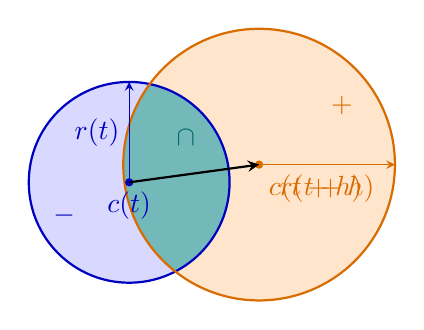
\begin{tikzpicture}[x=1.5cm,y=1.5cm,>=stealth]
 \fill[blue!15] (-.45,0) circle (.85);
 \fill[orange!20] (.65,.15) circle (1.15);
 \begin{scope}
  \clip (-.45,0) circle (.85);
  \fill[teal!55] (.65,.15) circle (1.15);
 \end{scope}
 \draw[blue!75!black,thick] (-.45,0) circle (.85);
 \draw[orange!85!black,thick] (.65,.15) circle (1.15);
 \fill[blue!75!black] (-.45,0) circle (1.5pt)
 node[below] {$c(t)$};
 \fill[orange!85!black] (.65,.15) circle (1.5pt)
 node[below right] {$c(t+h)$};
 \draw[->,thick] (-.45,0)--(.65,.15);
 \draw[blue!75!black,->] (-.45,0)--(-.45,.85)
 node[midway,left] {$r(t)$};
 \draw[orange!85!black,->] (.65,.15)--(1.8,.15)
 node[midway,below] {$r(t+h)$};
 \node[blue!75!black] at (-1.0,-.28) {$-$};
 \node[teal!80!black] at (.03,.38) {$\cap$};
 \node[orange!85!black] at (1.35,.65) {$+$};
\end{tikzpicture}
\caption{Przesunięcie środka i zmiana promienia
kuli (przekrój płaski). Część niebieska zostaje
usunięta, pomarańczowa dodana, a zielona
pozostaje wspólna dla obu dziedzin.
Znaki dotyczą zmiany dziedziny, nie znaku
funkcji podcałkowej.}
\label{ma2:fig:parameter-moving-ball}
\end{figure}

\section{Reguła Leibniza i ruchomy promień}

Dla funkcji skalarnej $w(t,s)$, gdzie $t$ należy
do otwartego $T\subseteq\R^m$, a $s\in[a,b]$
przy $a<b$,
załóżmy ciągłość $w$ i wszystkich $\partial_{t_i}w$
oraz różniczkowalność $\alpha,\beta:T\to[a,b]$.
Wtedy dla zorientowanej całki jednowymiarowej
\[
 L(t)=\int_{\alpha(t)}^{\beta(t)}w(t,s)\,
 \mathrm d\lambda_1(s)
\]
mamy
\[
 \partial_i L(t)=
 w(t,\beta(t))\partial_i\beta(t)
 -w(t,\alpha(t))\partial_i\alpha(t)
 +\int_{\alpha(t)}^{\beta(t)}
   \partial_iw(t,s)\,\mathrm d\lambda_1(s).
\]
Przy odwróconych końcach zapis oznacza ujemną całkę
po przedziale o uporządkowanych końcach.
Wzór jest zastosowaniem
\atlasref{AM1-32::ma1:thm:parameter-leibniz}{reguły Leibniza}
na prostej $t+h e_i$; ciągłość gwarantuje zgodność
całek Riemanna i Lebesgue'a. Jeżeli dodatkowo
$\alpha,\beta$ są klasy $C^1$, to prawe strony
są ciągłe w $t$: składniki brzegowe przez złożenie
funkcji ciągłych, a całkę z pochodnej przez
zbieżność zmajoryzowaną po przedłużeniu przez zero
na $[a,b]$ (funkcje charakterystyczne przedziałów
zbiegają poza ich końcami, a przy końcach równych
granica jest zero prawie wszędzie; przy odwróceniu
końców uwzględniamy znak). Dla ustalonego $t_0$
wybieramy zwartą kulę $K\subset T$ o środku $t_0$
i dodatnim promieniu. Ciągłość $\partial_{t_i}w$
na $K\times[a,b]$ zapewnia wspólne stałe ograniczenie,
całkowalne na $[a,b]$. Zatem $L\in C^1(T)$.

\begin{przyklad}[Różniczkowanie całki po kuli radialnej]
\label{ma2:ex:parameter-radial-leibniz}
Niech $h(t,r)$ i $\partial_t h(t,r)$ będą ciągłe
na $I\times[0,\infty)$, gdzie $I$ jest otwartym
przedziałem, a $\rho:I\to(0,\infty)$ różniczkowalna.
Zdefiniujmy
\[
 J(t)=\int_{B(0,\rho(t))}h(t,\|x\|_2)
 \,\mathrm d\lambda_n(x).
\]
Wzór radialny \ref{ma2:thm:improper-radial}
daje $J(t)=nv_n\int_0^{\rho(t)}h(t,r)r^{n-1}
\,\mathrm d\lambda_1(r)$.
W otoczeniu dowolnego $t_0$ promień jest
ograniczony przez pewne $R$; na $[0,R]$ możemy
zastosować jednowymiarową regułę Leibniza.
Otrzymujemy
\[
 \begin{split}
 J'(t)={}&nv_n\rho(t)^{n-1}h(t,\rho(t))\rho'(t)\\
 &+\int_{B(0,\rho(t))}\partial_t h(t,\|x\|_2)
 \,\mathrm d\lambda_n(x).
 \end{split}
\]
W drugim składniku użyliśmy ponownie wzoru radialnego.
W szczególności dla $h=1$ oraz $\rho(t)=t>0$
mamy $J'(t)=nv_nt^{n-1}$, zgodnie ze skalowaniem
objętości $J(t)=v_nt^n$.
Pierwszy składnik opisuje zmianę dziedziny,
drugi zmianę funkcji podcałkowej.
Wartości funkcji w punkcie $x=0$ nie wpływają na
wzór radialny, ponieważ $\lambda_n(\{0\})=0$.
Nie jest to jeszcze ogólny wzór różniczkowania
całki po ruchomej podrozmaitości.
\end{przyklad}


\paragraph{Wizualizacje interaktywne.}
Pierwszy wykres przedstawia przykład
\ref{ma2:ex:parameter-two-changes} dla $t=1$.
Dodajemy pomocniczy kierunek o długości $1$,
więc pola z rysunku są równe objętościom
odpowiednich graniastosłupów.
Suwak zmienia $h$ i pokazuje iloraz
różnicowy $5/2+3h/2+h^2/2$.
Drugi wykres przedstawia kule o środku
$c(h)=(h,0,0)$ i promieniu $1+h/2$.
Przezroczyste powierzchnie oznaczają
brzegi kul, a nie osobne miary powierzchniowe.
\begin{lstlisting}[language=Python]
import numpy as np
import plotly.graph_objects as go

faces=[(0,2,1),(0,3,2),(4,5,6),(4,6,7),
       (0,1,5),(0,5,4),(1,2,6),(1,6,5),
       (2,3,7),(2,7,6),(3,0,4),(3,4,7)]
i,j,k=zip(*faces)
def prism(a,b,lo,hi,color,name,visible):
    v=[(a,0,lo(a)),(b,0,lo(b)),(b,1,lo(b)),
       (a,1,lo(a)),(a,0,hi(a)),(b,0,hi(b)),
       (b,1,hi(b)),(a,1,hi(a))]
    x,y,z=zip(*v)
    return go.Mesh3d(x=x,y=y,z=z,i=i,j=j,k=k,
        color=color,name=name,visible=visible,
        showlegend=True)
hs=np.arange(1,9)/20
old=lambda x:1+x
fig=go.Figure(prism(0,1,lambda x:0,old,
    "#397db5","F(t)",True))
for jh,h in enumerate(hs):
    f=lambda x:1+(1+h)*x
    fig.add_trace(prism(0,1,old,f,
        "#15988c","Density",jh==4))
    fig.add_trace(prism(1,1+h,lambda x:0,f,
        "#d97706","Domain",jh==4))
steps=[dict(label=f"{h:.2f}",method="update",
    args=[dict(visible=[True]+
          [j==ih for j in range(len(hs)) for _ in range(2)]),
          dict(title=f"Q = {2.5+1.5*h+.5*h*h:.4f}")])
       for ih,h in enumerate(hs)]
fig.update_layout(sliders=[dict(active=4,steps=steps)],
    title="Q = 2.9062")
fig.write_html("am2_28_leibniz.html", include_plotlyjs=True)

p,q=np.meshgrid(np.linspace(0,np.pi,33),
                np.linspace(0,2*np.pi,65))
def sphere(c,r,color,visible):
    return go.Surface(x=c+r*np.sin(p)*np.cos(q),
        y=r*np.sin(p)*np.sin(q),z=r*np.cos(p),
        colorscale=[[0,color],[1,color]],
        opacity=.38,showscale=False,visible=visible)
fig=go.Figure(sphere(0,1,"#397db5",True))
for ih,h in enumerate(hs):
    fig.add_trace(sphere(h,1+h/2,"#d97706",ih==4))
steps=[dict(label=f"{h:.2f}",method="update",
    args=[dict(visible=[True]+[j==ih for j in range(len(hs))])])
       for ih,h in enumerate(hs)]
fig.update_layout(scene_aspectmode="cube",
    sliders=[dict(active=4,steps=steps)])
fig.write_html("am2_28_moving_ball.html", include_plotlyjs=True)
\end{lstlisting}

\section{Kontrola ogonów i dobór metody}

Na zbiorze nieograniczonym lub w pobliżu osobliwości
można zastąpić poszukiwanie wspólnej majoranty
jednostajną kontrolą ogonów. Dokładna teza i dowód
znajdują się w
\atlasref{ME-11::thm:tails-11}{teorii miary i całki}.
Jeżeli $(A_j)$ jest rosnącym wyczerpaniem mierzalnym
zbioru $A$ w sensie definicji
\ref{ma2:def:integral-exhaustion}, całki po $A_j$
są ciągłe względem parametru w $t_0$,
a dla pewnego otoczenia $V$ punktu $t_0$
\[
 \sup_{t\in V}\int_{A\setminus A_j}|f(t,x)|
 \,\mathrm d\lambda_n(x)\longrightarrow0,
\]
to przy całkowalności przekrojów na każdym $A_j$
całka na $A$ istnieje dla $t\in V$ i jest ciągła
w $t_0$. Wyczerpania można dobierać zgodnie
z rozdziałem \ref{ma2:ch:improper-euclidean}.
W przypadku stałego obszaru nieograniczonego
możemy przykładowo wziąć $A_j=A\cap[-j,j]^n$.
Gdy mamy wspólną całkowalną majorantę $g$ na $V$,
warunek kontroli ogonów jest automatyczny, ponieważ
\[
 \sup_{t\in V}\int_{A\setminus A_j}|f(t,x)|\,
 \mathrm d\lambda_n(x)
 \le\int_{A\setminus A_j}g(x)\,\mathrm d\lambda_n(x)
 \longrightarrow0
\]
na mocy twierdzenia \ref{ma2:thm:improper-exhaustion}.
Sama kontrola ogonów nie zastępuje jednak założenia
o ciągłości całek na poszczególnych $A_j$.

W kolejnych rozdziałach będziemy stosować te
narzędzia do całek wielokrotnych i całek
na podrozmaitościach przestrzeni euklidesowej.
